%%% LaTeX Template: Article/Thesis/etc. with colored headings and special fonts
%%%
%%% Source: http://www.howtotex.com/
%%% Feel free to distribute this template, but please keep to referal to http://www.howtotex.com/ here.
%%% February 2011

%%%%% Preamble
\documentclass[10pt,a4paper]{article}

\usepackage[T1]{fontenc}
\usepackage[bitstream-charter]{mathdesign}

\usepackage[utf8]{inputenc}% Input encoding
\usepackage{amsmath}	% Math

\usepackage{xcolor}
\definecolor{bl}{rgb}{0.0,0.2,0.6} 

\definecolor{background-image}{rgb}{1.0,0.9,0.7} 

% Translating the section, part, ... names into French
\usepackage[french]{babel}

% Setup the margins
\usepackage{geometry}
\newgeometry{margin=2cm}

% Customize the hyperlinks
\usepackage{hyperref}
\hypersetup{
    bookmarks=true,         % show bookmarks bar?
    unicode=false,          % non-Latin characters in Acrobat’s bookmarks
    pdftoolbar=true,        % show Acrobat’s toolbar?
    pdfmenubar=true,        % show Acrobat’s menu?
    pdffitwindow=false,     % window fit to page when opened
    pdfstartview={FitH},    % fits the width of the page to the window
    pdftitle={My title},    % title
    pdfauthor={Author},     % author
    pdfsubject={Subject},   % subject of the document
    pdfcreator={Creator},   % creator of the document
    pdfproducer={Producer}, % producer of the document
    pdfkeywords={keyword1} {key2} {key3}, % list of keywords
    pdfnewwindow=true,      % links in new window
    colorlinks=true,       % false: boxed links; true: colored links
    linkcolor=bl,          % color of internal links (change box color with linkbordercolor)
    citecolor=green,        % color of links to bibliography
    filecolor=magenta,      % color of file links
    urlcolor=bl           % color of external links
}

% For getting the caption on the side of an image
\usepackage{calc}
\usepackage{graphicx}
\usepackage{floatrow}
\floatsetup{style=ruled,footposition=caption}

\newcommand{\myfig}[2]{
\begin{figure}[htbp]
\floatbox[{\capbeside\thisfloatsetup{capbesideposition={right,top},capbesidewidth=4cm}}]{figure}[\FBwidth]
         {\caption{#2}\label{fig:#1}}
         {\includegraphics[width=5cm]{#1}}
\end{figure}
}


%\usepackage{sidecap}

\usepackage{sectsty}
\usepackage[compact]{titlesec} 
\allsectionsfont{\color{bl}\scshape\selectfont}

%%%%% Definitions
% Define a new command that prints the title only
\makeatletter							% Begin definition
\def\printtitle{%						% Define command: \printtitle
    {\color{bl} \centering \huge \sc \textbf{\@title}\par}}		% Typesetting
\makeatother							% End definition

\title{Machine Learning \\ 
		\large \vspace*{-10pt} Notes on A. Ng lectures\vspace*{10pt}}

% Define a new command that prints the author(s) only
\makeatletter							% Begin definition
\def\printauthor{%					% Define command: \printauthor
    {\centering \small \@author}}				% Typesetting
\makeatother							% End definition

\author{%
	Jérémy Fix \\
	Jeremy.Fix@Supelec.fr \\
	\vspace{20pt}
	}

% Custom headers and footers
\usepackage{fancyhdr}
	\pagestyle{fancy}					% Enabling the custom headers/footers
\usepackage{lastpage}	
	% Header (empty)
	\lhead{}
	\chead{}
	\rhead{}
	% Footer (you may change this to your own needs)
	\lfoot{\footnotesize }
	\cfoot{}
	\rfoot{\footnotesize page \thepage\ / \pageref{LastPage}}	% "Page 1 of 2"
	\renewcommand{\headrulewidth}{0.0pt}
	\renewcommand{\footrulewidth}{0.4pt}

% Change the abstract environment
\usepackage[runin]{abstract}			% runin option for a run-in title
\setlength\absleftindent{30pt}		% left margin
\setlength\absrightindent{30pt}		% right margin
\abslabeldelim{\quad}						% 
\setlength{\abstitleskip}{-10pt}
\renewcommand{\abstractname}{}
\renewcommand{\abstracttextfont}{\color{bl} \small \slshape}	% slanted text


% Pour gérer les lettrines
\usepackage{lettrine}

%%%%%%%%%%%%%%%%%%%%%%%%%%%%%%%%%%%%%%%%%%%%%%%%%%%%%%%%%%%%%%%%%%%%%%%%%%
%%% Start of the document
%%%%%%%%%%%%%%%%%%%%%%%%%%%%%%%%%%%%%%%%%%%%%%%%%%%%%%%%%%%%%%%%%%%%%%%%%%
\begin{document}
%%% Top of the page: Author, Title and Abstact
\printtitle 

\printauthor

\begin{abstract}
Notes on the Machine Learning lectures of A. Ng.
\end{abstract}

\tableofcontents

\pagebreak

\section{Linear regression with one or multiple variables}

\section{Logistic Regression}

We focus on classification problems for which the output $y$ is binary
(bi-class classification problem, later on, we will speak about
multiclass classification): $y \in \{0, 1\}$. We call class-0
the negative class and class-1 the positive class but these are just
arbitrary names. For example, one may seek to learn to classify a
tumor to be malignant or not depending on its size, or filter mails as
being spam or not depending on some measure.\\

With linear regression, we can define a boundary condition saying :
``if $h_\theta(x)$ is larger or equal than $0.5$ then consider it as
belonging to class-1, otherwise it belongs to class-0''.

Note:  il utilise le problème de classer des tumeurs, en ajoutant un
outlier tends à déplacer la frontière de décision pour donner un
mauvais classifieur. ``I would not use linear regression for
classification problems''. 

Il introduit la régression logistique pour contenir l'hypothèse
$h_\theta(x)$ dans $[0, 1]$ alors qu'avec la régression linéaire peut
donner des valeurs bien au dela de ce domaine alors que les étiquettes
valent disont $0$ et $1$... Mais il y a aussi la sensibilité aux
outliers(\textbf{à vérifier!!})\\


On introduit le modèle de régression logistique:
\begin{eqnarray}
h_\theta(x) &=& g(\theta^T x) = \frac{1}{1 + e^{-\theta^T x}}
\end{eqnarray}

On peut voir $h_\theta(x)$ comme la probabilité estimée que $y=1$ pour
l'entrée $x$. C'est à dire qu'on considère $h_\theta(x)$ comme un
modèle paramétré de $P(y=1 | x ; \theta)$. Pour trancher si une
entrée $x$ appartient à l'une ou l'autre des classes, il faut
introduire un seuil sur cette probabilité. Par exemple, si on prédit
$y=1$ quand $h_\theta(x) \geq 0.5$, cela correspond à prédire $y=1$
quand $\theta^T x \geq 0$. Le plan correspondant à $\theta^T x = 0$
est appelée ``decision boundary''. Comme le feature vector peut
contenir des combinaisons non-linéaires de nos observations, e.g.  $x
= [1, x_1, x_2, x_1^2, x_2^2]$, la boundary decision peut être
non-linéaire quand tracée dans l'espace des observations, e.g. $x_1,
x_2$.\\


On doit maintenant dériver des algorithmes pour trouver les paramètres
$\theta$. Partant d'une base d'apprentissage $(x^{(i)}, y^{(i)})$ avec
$\forall i, y^{(i)} \in \{0, 1\}$, on cherche les paramètres
$\theta$. Pour la régression linéaire, on a quantifié la
classification par une fonction quadratique $J(\theta) = \frac{1}{2m}
\sum_i (h_\theta(x^{(i)}) - y^{(i)})^2 =
\frac{1}{m}\sum_i \mbox{cost}(h_\theta(x^{(i)}), y^{(i)})$. La
fonction de coût est donc une fonction des coûts de chaque
exemple. Pour la régression linéaire, avec un coût quadratique, le
coût $J(\theta)$ était convexe et le problème d'optimisation avait
donc un seul minimum. Avec une hypothèse $h_\theta$ logistique, la
fonction de coût n'est plus convexe si on utilise un coût
quadratique ce qui a la conséquence fâcheuse d'introduire plusieurs
minimums locaux à la fonction de coût (ce qui pose des problèmes pour
la minimiser avec, par exemple, une descente de gradient). Pour la
régression logisitique, on introduit le coût logarithmique~:
\begin{equation}
\mbox{cost}(h_\theta(x), y) = \begin{cases} -\log(h_\theta(x)) & \mbox{
    si } y=1\\
-\log(1 - h_\theta(x)) & \mbox{ si } y=0
\end{cases}
\end{equation}
On remarque qu'on peut réécrire cette fonction de coût\footnote{On aurait pu imaginer une autre
  formulation de la fonction de coût $\mbox{cost}(h_\theta(x),y) = -\log((1-y)(1-h_\theta(x)) + y
h_\theta(x))$ \textbf{mais} il y a des raisons théoriques pour
préférer la version du texte, elle est convexe et est dérivée de
principe de Maximum Likelihood estimation \textbf{??????} } sous la forme
$\mbox{cost}(h_\theta(x),y) = -(1-y)\log(1-h_\theta(x)) - y
\log(h_\theta(x))$. Cette fonction de coût est \mbox{convexe} et donc sans
minimums locaux. On en vient à introduire la fonction de coût
$J(\theta)$~:
\begin{eqnarray}
J(\theta) &=& \frac{1}{m}\sum_i \mbox{cost}(h_\theta(x^{(i)}),
y^{(i)})\\
&=& -\frac{1}{m} \left( \sum_{i=1}^m y^{(i)} \log(h_\theta(x^{(i)})) +
(1 - y^{(i)}) \log(1 - h_\theta(x^{(i)}))\right)
\end{eqnarray}
Pour trouver les paramètres qui minimise cette fonction de coût, on
peut considérer une descente de gradient~:
\begin{equation}
\theta_j \leftarrow \theta_{j} - \alpha \frac{\partial}{\partial \theta_j} J(\theta)
\end{equation}
En calculant le gradient du coût par rapport aux paramètres, on
obtient la règle de mise à jour des paramètres~:
\begin{equation}
\theta_j \leftarrow \theta_{j} - \alpha \sum_{i=1}^m
(h_\theta(x^{(i)}) - y^{(i)}) x_j^{(i)}
\end{equation}
Comme pour la régression linéaire, les paramètres sont mis à jour
simultanément. On pourra remarquer que cette règle de mise à jour est identique à la
règle de mise à jour des paramètres pour la régression linéaire, à
ceci près que l'hypothèse $h_\theta$ est différente (et la fonction de
coût a été particulièrement bien choisie). Comme pour la régression
linéaire, on peut ajuster l'échelle des features (feature scaling)
pour améliorer la vitesse de convergence de la descente de gradient.\\


\textbf{Tracer} la fonction de coût quand $y=1$ pour montrer que si
$h_\theta(x)$ tend vers 1, le coût tends vers 0; Au contraire si
$h_\theta(x)$ tends vers 0 (alors que $y=1$ puisque que $h_\theta(x) =
P(y=1|x; \theta)$), le coût tends vers l'infini et l'algorithme est
donc fortement pénalisé pour cette erreur. On peut mener un
raisonnement similaire pour le cas $y=0$ dans lequel on pénalise
fortement lorsque $h_\theta(x) \rightarrow 1$.\\

La descente de gradient est une des manières de minimiser notre
fonction de coût. Il en existe d'autres, parfois plus rapide en terme
du nombre d'itérations nécessaires pour atteindre le minimum. Une
liste d'algorithmes alternatifs est donnée ci-dessous~:
\begin{itemize}
\item gradient conjugué
\item BFGS
\item L-BFGS
\end{itemize}
Ces algorithmes ont un certain nombre d'avantages par rapport à la
descente de gradient:
\begin{itemize}
\item il n'y a pas besoin de spécifier manuellement un taux
  d'apprentissage $\alpha$, celui-ci est ajusté automatiquement
\item ils sont en général plus rapide à converger qu'une descente de
  gradient
\end{itemize}
Ils sont néanmoins plus compliqués à comprendre et mettre en
{\oe}uvre. Cela dit, il existe un certain nombre d'implémentations
clé-en-main de ces algorithmes. \\

With Octave, you would make use of the \emph{fminunc} function with
specific options setting which algorithm to use.

% options = optimset('GradObj', 'on', 'MaxIter', '100');
% initialTheta = zeros(2, 1);
% [optTheta, functionVal, exitFlag] = fminunc(@costfunction,
% initialTheta, options)
% where [jVal, gradient] = costfunction(theta) returns the value of
% the function and its gradient 


We now go back to multi-class classification. Therefore, we suppose
that the output $y$ can take more than two values. One way to solve
this problem is to consider multi-class classification problems as
multiple binary classification problems. We then train as many binary
classifiers as we have classes. Each of these classifier learns to
recognize one class versus all the others. Given all the individual
classifiers $h_i$, we may define label an input $x$ as belonging to
the class which maximizes the outputs $h_i(x), \forall i \in
[1..k]$.\\

\section{Regularization}

\subsection{Motivation}

Sometimes, when trying to fit an hypothesis to a data set, we may run
into a problem called overfitting. Overfitting arises because we have
just a partial observation of the true model that generates the data
we are trying to fit. We therefore make an hypothesis on the shape of
this model. Obviously, when we fit a model on a dataset, we want to
interpolate the output for unobserved inputs (inputs that are not in
the training set). The hypothesis we consider define how different we
can interpolate this output. The simplest example of overfitting can
be seen when fitting a polynomial on data set. If we increase the
degree of the polynomial, we introduce more flexibility to the model
(indeed, with the Lagrange polynomials, we know that we can fit
perfectly any data set if we don't constrain the degree of the
polynomial). This flexibility can lead to more variability in the
model which may impairs the ability of the model to generalize,
i.e. to give the right answer on new data unavailable in the training
set.\\

There are two options to adress overfitting. The first one is to
reduce the number of features whether by manually selecting the
features to keep or to use model selection algorithm. However,
throwing away some features may throw away some information contained
in the dataset. The second option is called
regularization. Regularization is a technique which allows to balance
the tendency to overfit the training set by a term which constrains
the \emph{complexity} of the model.\\

\textbf{Des données à fiter avec un polynôme}\\

Suppose we consider linear regression with some polynomials of the
inputs~:$h_\theta(x) = \theta_0 + \theta_1 x + \theta_2 x^2 + \theta_3
x^3 + \theta_4 x^4$. If we penalize the two parameters $\theta_3$ and
$\theta_4$, the polynomial $h_\theta$ will be simpler. To penalize
these two parameters we can modify the quadratic cost function by
adding terms that increases the cost depending on the amplitude of
these parameters, e.g. $J(\theta) = \frac{1}{m} (h_\theta(x^{(i)}) -
y^{(i)})^2 + 1000 \theta_3^2 + 1000 \theta_4^2$. Minimizing this
modified cost function will constrain the parameters $\theta_3$ and
$\theta_4$ to be small. More generally, as we may not know which
parameters influence overfitting, we introduce the following cost
function for linear regression~:
\begin{equation}
J(\theta) = \frac{1}{2m} \sum_{i=1}^m (h_\theta(x^{(i)}) -
y^{(i)})^2 + \lambda \sum_{i=1}^{n} \theta_j^2
\end{equation}
By convention, $\theta_0$ is not regularized. The parameter $\lambda$
balances the trade off between fitting the dataset and keeping the
parameters $\theta_i$ small. If $\lambda$ is set too large,
minimization of this cost function may unfortunately lead to
underfitting, i.e. we even do not fit the training set. Fortunately,
one may define algorithms automatically adjusting the penalization
coefficient $\lambda$.\\


\textbf{Question} : est ce qu'introduire le terme de régularization ne
rends pas la fonction de coût non convexe ? NON d'après une question
du quizz, la fonction de coût reste convexe.\\

\textbf{Question} : pourquoi est ce qu'on s'en fout de ne pas
régularizer le terme $\theta_0$.\\

\textbf{Question} : pourquoi ne pas pénaliser plus les termes de grand degré?

\subsection{Regularized linear regression}

We remind the cost function for linear regression with L2
regularization~:
\begin{equation}
J(\theta) = \frac{1}{2m} \sum_{i=1}^m (h_\theta(x^{(i)}) -
y^{(i)})^2 + \lambda \sum_{i=1}^{n} \theta_j^2
\end{equation}

Considering this regularized cost function, one must modify the
gradient descent algorithm. The update of the parameters now reads~:

\textbf{TODO, calculer le gradient, d'après Ng } : $ \theta_0
\leftarrow \theta_0 - \alpha/m \sum_{i=1}^m (h_\theta(x^{(i)})
-y^{(i)}) x_0^{(i)} ; \forall j\neq 0, \theta_j
\leftarrow \theta_j - \alpha ( 1/m \sum_{i=1}^m (h_\theta(x^{(i)})
-y^{(i)}) x_j^{(i)} + \lambda/m \theta_j) = (1 - \alpha \lambda/m)
\theta_j - \alpha / m ...$.

By isolating the terms depending on $\theta_j$, one gets an update
rule of the form $ \theta_j \leftarrow \beta \theta_j - \alpha/m ..$,
we see that we shrink the parameter and move in a direction minimizing
the cost function (when considered without the regularization term).\\

We also saw that we can use normal equations for solving linear
regression. Without regularization, the optimal parameters using
normal equation was :$\theta = (X^T X)^{-1} X^T y$. We regularization
inside, the normal equation now reads $\theta = (X^T X + \lambda
R)^{-1} X^T y$ where $R$ is a diagnoal matrix filled in with $1$,
except for the first element which is set to $0$. For e.g., with
$n=2$, $R = [0 0 0; 0 1 0; 0 0 1]$.\\

If you have less examples than features, the matrix $X^TX$ is non
invertible. If you use regularization, it is possible to prove that
the matrix $X^T X + \lambda R$ cannot be singular and that you can
always invert it.\textbf{AH OUAIS ???}.\\


\subsection{Regularized logistic regression}

For logistic regression, the cost function reads~:
\begin{equation}
J(\theta) = -\frac{1}{m} \sum_{i=1}^m (y^{(i)} \log(h_\theta(x^{(i)}))
+(1-y^{(i)}) \log(1 - h_\theta(x^{(i)}))) 
\end{equation}
We can also add L2 regularization to this cost function to get~:
\begin{equation}
J(\theta) = -\frac{1}{m} \sum_{i=1}^m (y^{(i)} \log(h_\theta(x^{(i)}))
+(1-y^{(i)}) \log(1 - h_\theta(x^{(i)}))) + \lambda/(2m) \sum_j \theta_j^2
\end{equation}

The gradient descent update is then modified into $ \theta_0
\leftarrow \theta_0 - \alpha/m \sum_{i=1}^m (h_\theta(x^{(i)})
-y^{(i)}) x_0^{(i)} ; \forall j\neq 0, \theta_j
\leftarrow \theta_j - \alpha ( 1/m \sum_{i=1}^m (h_\theta(x^{(i)})
-y^{(i)}) x_j^{(i)} + \lambda/m \theta_j) = (1 - \alpha \lambda/m)
\theta_j - \alpha / m ...$.\\

The update is very similar to regularized linear regression but remind
that the hypothesis $h_\theta$ is different for logistic regression.


\section{Idées de démos}

Pour la régularisation, une appli dans laquelle on fit un polynôme sur
des données et on règle dynamiquement la contribution $\lambda$ de la
régularisation pour voir la forme du modèle appris.\\


\section{Neural Networks: Representation}

\textbf{A vérifier : overfitting if we increase the number of features
  with a constant number of data ?}\\



Neural networks are the state of the art technique for several machine
learning problems. To motivate neural networks, let us consider a
non-linear classification problem. As we saw, we can use logistic
regression with polynomial features (say $x_1 x_2, x_2^3 x_3,
..$). However, given the size of our inputs, the size of the feature
vector may be a polynomial of it which will certainly be quite big and
increase the tendency to overfitting (if we consider too many features
relative to the number of the data we have, we can easily encounter
overfitting). To give on example, if one considers object recognition
from images of size $50 \times 50$, one obtains images with $n=2500$
pixels. If we just consider only quadratic terms $x_i x_j$, one gets
around $3$ million features, the number of features is indeed
$n^2/2$. One may limit the number of features, but this selection
is, there, somehow arbitrary. Neural networks are a much better way to
define non-linear hypotheses than logistic regression with polynomial
features.\\


Neural networks, while originally derived from the desire to mimick
the brain, is used from an abstract viewpoint in Machine Learning
where we consider simple massively interconnected entities. Each
entity receives signal from others, process it locally and transmit a
signal to other entities. The simple model we consider is a logistic
unit, which receives inputs denotes $x_i$, computes a weighted sum of
it and apply a sigmoid transfer function on it. This is nothing more than what
we saw in the previous section $y = h_\theta(x) = \frac{1}{1 +
  e^{-\theta^T x}}$. We also add a bias unit to the inputs $x_0 = 1$
in addition to the signals received from the other neurons $x_i, i
\geq 1$. In the neural network literature, $\theta$ are called the
weights. We can build layers of such units and interconnect them. A
multilayer neural network is shown on fig.\ref{fig:neunet}.

\begin{figure}[htbp]
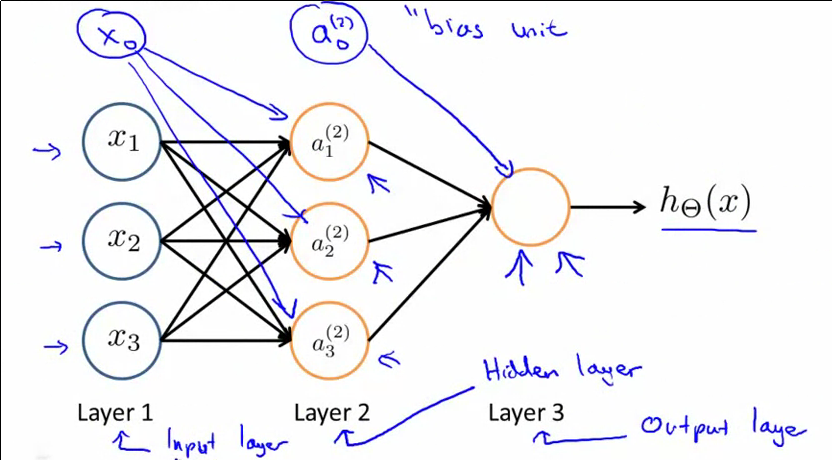
\includegraphics[width=0.7\columnwidth]{Figs/neunet.png}
\caption{\label{fig:neunet} Representation of a feedforward neural
  network. Capture from the A. Ng lecture.}
\end{figure}

We will denote $a_i^{(j)}$ the activation of the i-th unit of j-th
layer. We denote $\theta^{(j)}$ the matrix of weights from layer $j$
to layer $j+1$\footnote{We here consider only feedforward neural
  networks were the connections always go from layer $j$ to layer
  $j+1$}. The activation is computed according to~:
\begin{equation}
\begin{cases}
\forall i \geq 1, \forall j>1, a_i^{(j)} &= g(z_i^{(j)})\\
\forall i \geq 1, \forall j>1, z_i^{(j)} &= \sum_k \theta_k^{(j-1)} a_k^{(j-1)}\\
\forall i \geq 1, a_i^{(1)} &= x_i\\
\forall j, a_0^{(i)} &= 1
\end{cases}
\end{equation}
These equations tell nothing more than that the first neuron is the
bias for the next layer, the activations $a_i^{(1)}$ of the first layer equal our
inputs and each neuron in a subsequent layer computes its activation $a_i^{(j)}$
as a sigmoid of a weighted sum of the activations of the previous
layer $a_k^{(j-1)}$. A vectorized notation for computing the activations of layer
$j+1$ is simply $a^{(j+1)} = g(\theta^{(j)} . a^{(j)})$ where
$\theta^{(j)}$ is a matrix of size $|L_{j+1}| \times |L_{j}|$ with
$|L_j|$ the number of neurons in layer $j$ (the bias being
included). For regression, the last layer contains a single neuron of
which the activation, if unfolded, is a function of the input
$x$. Computing the activations in a layer-wise manner from the very
first layer to the output is called the forward propagation. If we
take a closer look to the 3-layers neural network depicted above, the
hidden to output layer is nothing more than a logistic regression with
Layer 2 representing the features. Now, if we include the very first
layer with the weights projecting the inputs to the hidden layer, we
can see it as building the features feeding the logistic
regression. And the nice thing there is that the features are learned
through the weights from Layer 1 to Layer 2. It may not be completely
clear that the features we compute that way (the activations of layer
1) can be arbitrary polynomials but indeed one may demonstrate that if
we don't restrict ourselves to a single hidden layer, one can
approximate any function (feedforward neural networks are universal
approximators) so that feedforward neural networks have at least the
expressiveness of logistic regression.\\

Now let us consider simple binary operations like and, or, not, xor. We can
easily write a simple neural network with a single input layer and a
single output for the and and \emph{or} functions :
\begin{itemize}
\item \emph{and} function : $\theta =(-30, 20, 20)$
\item \emph{or} function : $\theta =(-10, 20, 20)$
\item \emph{not} function : $\theta =(10, -20)$
\end{itemize}
These are both linearly separable problems. The Xor function is not
linearly separable and one needs to consider at least one hidden layer
to compute it. To put it simply, we just need to write $x_1 \mbox{xor}
x_2 = \mbox{or}(\mbox{and}(\mbox{not}(x1),x_2),
\mbox{and}(x1,\mbox{not}(x_2)))$. The functions not(x1) or x2, as well
as x1 and not(x2) can be compute with a single layer. These are the
input to hidden layer connections. Finally, we just connect the hidden
to the output layer for computing the or function.\\

Before, we were speaking about a simple regression example. An example
of multi-class classification is given by the LeNet 5 feedforward
neural network developed by Y. LeCun which he trained for recognizing
handwritten digits. The trained network is quite unsensitive to scale,
orientation, and some forms of noise. For multi-class classification,
we consider an output layer of the size of the number of classes. The
output $y^{(i)}$ for input $x^{(i)}$ is set to $y^{(i)}_j = \delta(j,
l^{(i)})$ where $\delta$ is the kronecker symbol and $l^{(i)}$ is the
class of the input $x^{(i)}$.




\textbf{Ref pour l'approximateur universel?}

\section{10}

In this section, few advices are given so as to know on which parameters one must play in order to improve the performances of the machine learning algorithm.\\

For example, when we test an hypothesis and find that it performs very badly on new unknown data, there are indeed various options one may be tempted to try, among which :
\begin{itemize}
\item get more training examples, it will probably better constrain the optimization of the hypothesis
\item try smaller sets of features to avoid overfitting
\item try getting additional features
\item try adding polynomial features
\item try decreasing or increasing the regularization parameter $\lambda$
\end{itemize}
Instead of trying one of these options at random, we can diagnose what is going wrong with our algorithm. One possibility to diagnose how an hypothesis performs is, in low dimension (up to 3), to plot the decision boundary for classification or the hypothesis directly for regression. However, in higher dimensions, this is not possible. \\

\subsection{Training set/Test set and error measures}
We would rather split the dataset in (at least) two datasets : a \textbf{training set} (70\% of the data) and a \textbf{test set} (30 \% of the data).\footnote{be sure that these sets are made of random samples of the datasets to avoid training on a specific region of the space while testing on another non-overlapping region}. Then we optimize the parameters on the training set and measure the generalization error on the test set. For classification problems, one may also measure the misclassification error~:
\begin{equation}
\mbox{err}(h_\theta(x), y) = \begin{cases}
1 & \mbox{ if } h_\theta(x) \geq 0.5, y = 0\\
  & \mbox{ or } h_\theta(x) < 0.5, y = 1\\
0 & \mbox{ otherwise} 
\end{cases}
\end{equation}
The test classification error is then just the mean over the test set of the misclassification error above which represents the proportion of the test set that is misclassified.

\subsection{Model selection and train/validation/test sets}

As we know already, the training error alone is not an appropriate measure for evaluating the performances of an hypothesis on unseen data since we might be overfitting. Instead, we should use the test set error. Suppose we wish to select among several polynomial hypothesis one that performs better. To do such a model selection, we will compare the test set errors and select the model with the lowest test error; However, to report the generalization ability of the model that we selected, we should use additional data as using the test set might overestimate the generalization error of the model (the degree of polynomial was indeed selected so that the test set error is decreased). Therefore, we should split the dataset into three pieces : \textbf{the training set} (60\%), \textbf{the cross-validation (cv) or validation set} (20\%) and \textbf{the test set} (20\%):
\begin{itemize}
\item the training set is used to optimize the parameters of the models
\item the test set is used for selecting among the various that we have trained
\item the validation set is used to estimate the generalization error of the selected model
\end{itemize}

\subsection{Bias/variance issues}

High bias issue is when the hypothesis is not sufficiently complex (underfit) while high variance is when the hypothesis is too complex (overfit). To better appreciate these issues, let us consider the case of polynomial hypothesis and plot both the training and validation errors as function of the degree of the polynomial (fig.~\ref{fig:crossvalidation_training_errors}). \\

As we increase the degree of the polynomial, we expect the training error to decrease as the model is more and more complex and we can overfit the training set more easily with higher degrees. The cross validation error will usually start as high as the training error, decrease and, then , at some point, increase as we overfit the training set and impair the generalization ability of the hypothesis.\\

\begin{figure}[htbp]
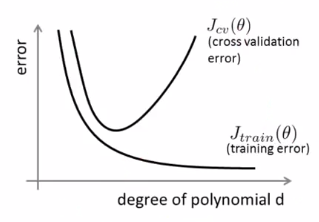
\includegraphics[width=0.5\columnwidth]{./Figs/crossvalidation_training_errors.png}
\caption{\label{fig:crossvalidation_training_errors}Typical curves of training and validation errors function of the degree of a polynomial hypothesis}
\end{figure}

Detecting whether we encounter a high variance or high bias problem is critical as we will not behave the same way in the two conditions. A high bias means a model that is not enough complex such that it cannot even fit the training set properly. A high variance means a model that is too complex so that it certainly fits perfectly the training set but performs poorly on the test set.

\begin{tabular}{|c|c|c|c|}
                &      & Validation error &      \\
                &      & Low              & High \\
\hline
Training error  & Low  & Good             & High variance \\
                & High &  -               & High bias \\
\end{tabular}


\subsection{Regularization and bias variance}

Varying the regularization parameter will affect the bias/variance. A very large parameter will penalize high values, leading to small parameters, leading to a high bias (fig.~\ref{fig:bias_variance_regularization}). If the regularization parameter is too small, say absent, a model that is too complex will not be penalized and we will probably run into high variance issues. Therefore, the regularization parameter must be correctly adjusted. This parameter must be choosen empirically, by testing different values for this parameter and checking both the training and cross validation errors. We then peak out the parameter giving a the lowest cross validation error and then evaluate the true performances on the test set.


\begin{figure}[htbp]
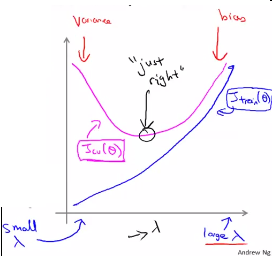
\includegraphics[width=0.5\columnwidth]{./Figs/bias_variance_regularization.png}
\caption{\label{fig:bias_variance_regularization} Skecthes of how the training and cross validation errors usually evolve as a function of the regularization parameter.}
\end{figure}

We can also plot the training and cross validation errors as functions of the number of training examples (\textbf{the learning curves}). The training error usually increases as you use a larger training set as it is pretty easy to fit perfectly few examples while more complicated to fit more. The cross validation error will usually decrease as you more easily overfit small training set and you generalize better if you use more training examples that better constrain the hypothesis.

\begin{itemize} 
\item if an algorithm is suffering from \textbf{high bias} (e.g. the hypothesis is not complex enough), getting \textbf{more training data will not help much}
\item if an algorithm is suffering from \textbf{high variance}, getting \textbf{more training data will help}
\end{itemize}

Given the previous observations, below is a list of options to consider depending on whether we face a high bias or high variance issue~:
\begin{itemize}
\item Getting more training examples : will help fixing high variance problems
\item try smaller sets of features: will help fixing high variance problems
\item try getting additional features: will usually help fixing high bias
\item try adding polynomial features : might help fixing high bias
\item try decreasing $\lambda$ for fixing high gbias, increasing $\lambda$ for fixing high variance
\end{itemize}

\section{Machine learning system design}

\subsection{Prioritizing what to work on : Spam classification example}

This section deals with various aspects of designing a machine learning system using the example of designing a spam classifier.\\


The first step is to decide what to use for the features. For example, we might use $100$ words that we consider might be indicative of the spam/non-spam category or to actually pike the words appearing the most frequently in the emails. The feature vector will then be a binary vector indicating whether a word appears or not in the email to classify. Some specific sophisticated features might also be added (e.g. from the header of the email, the body, checking for mispelled words, ...).\\

\subsection{Error analysis}

To design a machine learning system, one should 
\begin{enumerate}
\item start with a simple, quickly to implement, (dirty) algorithm and test it on a cross validation set
\item plot learning curves to decide whether we should focus on more data, more features, ...
\item error analysis : check which examples are misclassified from the cross validation set and why they are misclassified (what is particular about them)
\end{enumerate}

In particular, error analysis is really critical as it will really
help in adjusting the features to use. For spam classification, a
stemming software (e.g. Porter Stemmer) can be usefull for deciding
whether or not some variations of the same word should be considered
the same word. In this situation, there is no other solutions than
trying different solutions and comparing their performances with
respect to the cross-validation and test errors.

\subsection{Error metrics for skewed classes}

An important caveat can lead us to misinterpret the test
error. Imagine we train a classifier for deciding whether or not a
patient has a cancer. If we get a test error of 1\% we might say the
learning algorithm is doing pretty well. However, if the data are such
that only 0.5 \% of the patients have a cancer, the 1\% is actually
pretty high. We speak about \textbf{skewed classes} when the positive and
negative examples of the data are really unbalanced as it was the case
for the cancer data. Indeed, in such a situation, it is pretty easy to
design an efficient algorithm with respect to the test error: just
attribute the label of the largest class ! In such a situation, the usual
\textbf{classification error on the test set is not a sound error
  metric}. We rather introduce other measures : precision, recall,
accuracy, QUATIREME ELEMENT !!!! Suppose we work on a binary
classification task, we then introduce true/false positives and
true/false negatives according to the following table~:
\begin{tabular}{cccc}
& & Actual class & \\
& & 1            & 0 \\
Predicted class & 1 & True positive & False positive \\
                & 0 & false negative & true negative \\
\end{tabular}

The four measures are then defined as~:
\begin{eqnarray}
\mathrm{precision} &=& \frac{\mathrm{true\ positives}}{\mathrm{\#predicted\
  positive}} = \frac{\mathrm{true\ positives}}{\mathrm{true\
    positives}+\mathrm{false\ positives}}\\
\mathrm{recall} &=& \frac{\mathrm{true\ positives}}{\mathrm{\#actual\
  positives}} = \frac{\mathrm{true\ positives}}{\mathrm{true\
    positives}+\mathrm{false\ negatives}}
\end{eqnarray}
The \textbf{precision} indicates the fraction of the patients that are
positives among the patients classified as positives\footnote{by
  convention, when faced a classification problem with skewed classes,
the rare cases are the positive ones}. The
\textbf{recall} indicates the fraction of positive examples that were
correctly classified as positive. If we consider our example where the
algorithm classifies all the patients as not having a cancer, both the
recall and precision will be zero.

\subsection{Trading off precision and recall and $F_1$ score}

If we continue with our example of cancer classification and check the
influence of the decision threshold (say with a hypothesis
$0 \leq h_\theta(x) \leq 1$, we predict $1$ if $h_\theta(x) \geq T$
and $0$ if $h_\theta(x) < T$). If $T = 0.5$ we have a certain
precision and recall. If \textbf{we increase $T$}, say $T=0.9$, we will be much
more selective and much more confident about the examples that we
classify as positives. Therefore, the fraction of examples that are
really positives among the ones that we classify as positives will be
higher, then a \textbf{higher precision}. However, as much less examples are
classified as positives, the \textbf{recall will be lower}. If on the
opposite, we decrease the threshold, say $T=0.3$, we will be more
conservative as more than necessary patients will be classified as
positive, in which case we will have a \textbf{lower precision} and \textbf{a
higher recall}. Usually, there is a trade off between precision and
recall. Now, if we compare several algorithms (or the same with
different meta-parameters), they will have different precision $P$ and
recall $R$ values. To compare them, we introduce the $F_1$ score. As
we saw previously, some simple algorithms (like always assigning the
same class) is not a usefull classifier. Whether always saying ``class
0'' or ``class 1'', these algorithms will have whether high precision
and low recall or low precision and high recall. If we compute the
mean of precision and recall, it will be the same in the two
situations as well as the same as an algorithm which has equal
precision and recall. Therefore, the mean is not discriminative enough
for deciding which algorithm performs best. The $F_1 \in [0,1]$ score is rather
defined as~:
\begin{equation}
F = 2 \frac{P R}{P + R}
\end{equation}


\subsection{Data for machine learning}

\end{document}
